% RESULTADOS-------------------------------------------------------------------

\chapter{ANÁLISE E DISCUSSÃO DOS RESULTADOS}
\label{chap:resultados}

A conceitualização de qualidade é complexa dada sua subjetividade, o mesmo se aplica a qualidade de software. \cite{morais2010qualidade} escreve em seu trabalho que a qualidade está associada a uma série de ações que devem ser executas dentro de uma organização com o fim de criar um produto que satisfaça às expectativas dos clientes. \cite{morais2010qualidade} descreve ainda que no contexto de software a qualidade pode ser vista como um conjunto de características que devem ser criadas para satisfazer as necessidades do usuário.

Neste capítulo, são mostrados resultados da avaliação de qualidade da aplicação KeeMe. A Seção \ref{sec:lighthouse} irá abordar sobre os resultados da avaliação feita utilizando a ferramenta Lighthouse, que é representada em \cite{lighthouse} como uma ferramenta de testes automatizados de qualidade de páginas web, que mostra numa escala de 0 a 100 o quanto uma aplicação web segue determinados requisitos de qualidade.


\section{Avaliação de Qualidade Utilizando Lighthouse}
\label{sec:lighthouse}

Com já foi abordado, o Lighthouse, segundo \cite{lighthouse} se trata de uma ferramenta de código aberto que realiza testes automatizados de qualidade em páginas web. Seus critérios de avaliação são:

\begin{itemize}
    \item Desempenho: avalia o desempenho geral de uma página, como o tempo que leva para que ela seja carregada pela primeira vez, o tempo até que se possa interagir com os elementos da tela, entre outros fatores;
    \item Acessibilidade: se refere aos parâmetros de acessibilidade utilizados durante a criação do código HTML e da interface de uma página. Esses parâmetros são o tamanho da fonte, o contraste entre a cor das fontes e do plano de fundo, entre outros fatores;
    \item SEO (\textit{Search Engine Optimization}): avalia a capacidade que uma aplicação possui de ser indexada por um motor de busca, como o Google. Em outras palavras, se refere à capacidade que uma aplicação possui de poder ser encontrada por buscadores;
    \item Práticas Recomendadas: este critério está ligado ao índice de boas práticas que foram seguidas na construção da página. Essas boas práticas incluem não mostrar erros no console dos navegadores, tornar a página rápida, tornar a página segura, entre outros;
\end{itemize}

O Lighthouse avalia esses fatores, e então pontua de 0 a 100 a página web, mostrando também o que levou àquela nota. O \cite{lighthouse} classifica as notas como sendo: 0 a 49, como "Desempenho Pobre", ou seja, sem muita qualidade; 50 a 89, como "Necessita de Melhoria", significa que a aplicação possui qualidade, mas precisa ser melhorada; e de 90 a 100 como "Bom", ou seja, a aplicação possui qualidade no critério avaliado. Essa ferramenta foi utilizada por conta da necessidade de se ter uma avaliação precisa da qualidade da aplicação, além de se ter um norteador do que poderia ser feito para que possa ser melhorada.

A Figura \ref{fig:graficoResultadosDesktop} mostra a média de resultados da avaliação de todas as telas acessadas através de um computador, para isso, acessou-se cada uma das telas, fazendo uma avaliação da qualidade e registrando os resultados, esses resultados foram então somados e divididos pela quantidade total de telas proporcionando a média entre elas. Como é possível ver no gráfico, todos os resultados ficaram acima dos 90 pontos, indicando que a aplicação segue os melhores critérios de qualidade. O Desempenho foi pontuado com 96,63; já Acessibilidade 96,55; enquanto SEO 99,75; e Boas Práticas 100.

\begin{figure}[H]
    \centering
    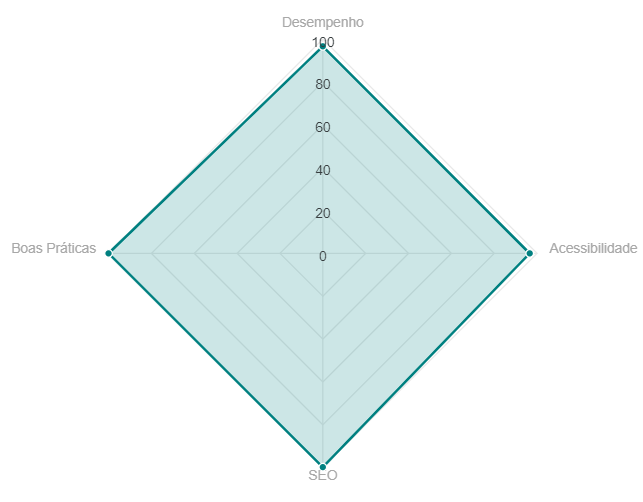
\includegraphics[width=12cm]{dados/figuras/Resultados/radar_desktop.png}
    \caption{Média de Resultados do Acesso por Computador}
    \label{fig:graficoResultadosDesktop}
\end{figure}

A Figura \ref{fig:graficoResultadosMobile} mostra a média de resultados da avaliação de todas as telas acessadas através de um dispositivo móvel, para se obter essa média foi realizado o teste de todas as telas do sistema através de um dispositivo móvel, após isso os resultados foram registrados, somados e divididos pela quantidade total de telas proporcionando a média de qualidade entre elas. Através do gráfico é possível ver que enquanto todos os outros resultados ficaram acima dos 90, o Desempenho ficou entre 70 e 80, o que indica que a aplicação possui um bom desempenho, mas que este ainda precisa ser melhorado no que diz respeito ao acesso por um dispositivo móvel. Sendo assim, as médias das notas foram: Desempenho, 75,27; Acessibilidade, 96,55; SEO, 99,75; e Boas Práticas, 99,75;

\begin{figure}[H]
    \centering
    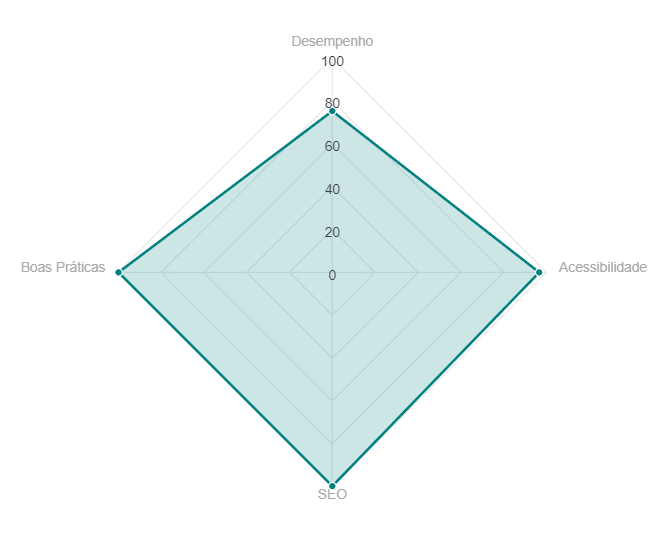
\includegraphics[width=12cm]{dados/figuras/Resultados/radar_mobile.png}
    \caption{Média de Resultados do Acesso por Dispositivo Móvel}
    \label{fig:graficoResultadosMobile}
\end{figure}

Como podemos ver nos resultados, a aplicação possui bons índices de qualidade tanto no acesso por um computador quanto no acesso por um dispositivo móvel. Como mostrado no gráfico da Figura \ref{fig:graficoResultadosMobile} o desempenho nos dispositivos móveis ainda precisa ser melhorado, tal resultado está ligado à utilização do React, ferramenta retratada em \cite{react} como sendo um \textit{framework} de criação de interfaces HTML usando Javascript. O React faz o carregamento de todo o \textit{script} gerado durante o primeiro acesso, para se melhorar a performance é necessário que seja feita uma estratégia de carregamento dinâmico desse \textit{script}.

